\documentclass[12pt, compress]{beamer}
\usetheme{m}

\usepackage{booktabs}
\usepackage[scale=2]{ccicons}

\usepgfplotslibrary{dateplot}

\title{Realization of an 802.15.4-like MAC layer with Mote Runner}
\subtitle{}
\date{\today}
\author{Andrea Salini - 231413 \\ Lorenzo Di Giuseppe - 227515 \\ Matteo Gentile - 230997}
\institute{DISIM - Università degli Studi dell’Aquila}

\begin{document}

  \maketitle
  
\begin{frame}[fragile]
  \frametitle{Introduction}
  \begin{itemize}
    \item Object of this project is the exploration of Mote Runner, an IBM’s infrastructure platform for WSN
    \item For a deep understanding of MR the focus of this works was the design and develop of a 802.15.4-like MAC layer
    \item Oscilloscope is an applications developed to test the MAC layer
    \item The application was tested on IRIS mote
  \end{itemize}
\end{frame}

\begin{frame}[fragile]
  \frametitle{Index}
  \begin{itemize}
    \item Introduction to Mote Runner
    \item Testing Mote Runner
    \item A MAC Layer in Mote Runner
    \item 6LoWPAN implementation in Mote Runner
    \item Conclusion
  \end{itemize}
\end{frame}

\section{Introduction to Mote Runner}
\begin{frame}[fragile]
  \frametitle{Mote Runner}
  \begin{itemize}
    \item An OS and a runtime and development environment for WSN
    \item Key features:
    \begin{itemize}
      \item Support for RT constraints \& energy awareness
      \item Portability thanks to a VM that abstracts the HW
      \item Event oriented programming paradigm
      \item High level coding (Java - C\#)
      \item Debugging \& simulation environments
    \end{itemize}
    \item It’s still in beta and is evolving towards IoT
  \end{itemize}
\end{frame}

\begin{frame}[fragile]
  \frametitle{Mote Runner}
  \begin{columns}
    \begin{column}{.48\linewidth}
    	
    \end{column}
    \hfill
    \begin{column}{.5\linewidth}
    	\begin{figure}
	  \centering
	  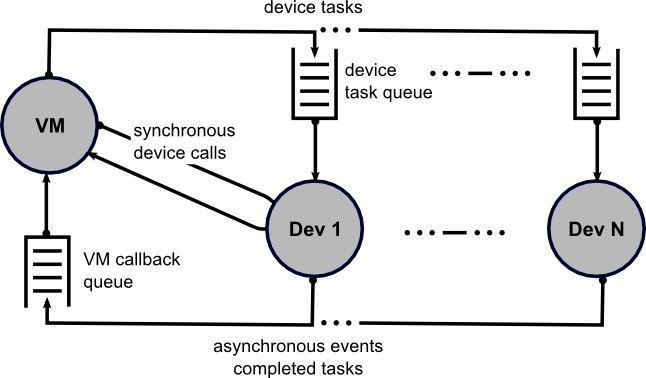
\includegraphics[width=\textwidth]{img/vm-dev.jpg}
    	\end{figure}
    \end{column}
  \end{columns}
\end{frame}

\begin{frame}[fragile]
  \frametitle{Mote Runner}
  \begin{columns}
    \begin{column}{.5\linewidth}
    	\begin{figure}
	  \centering
	  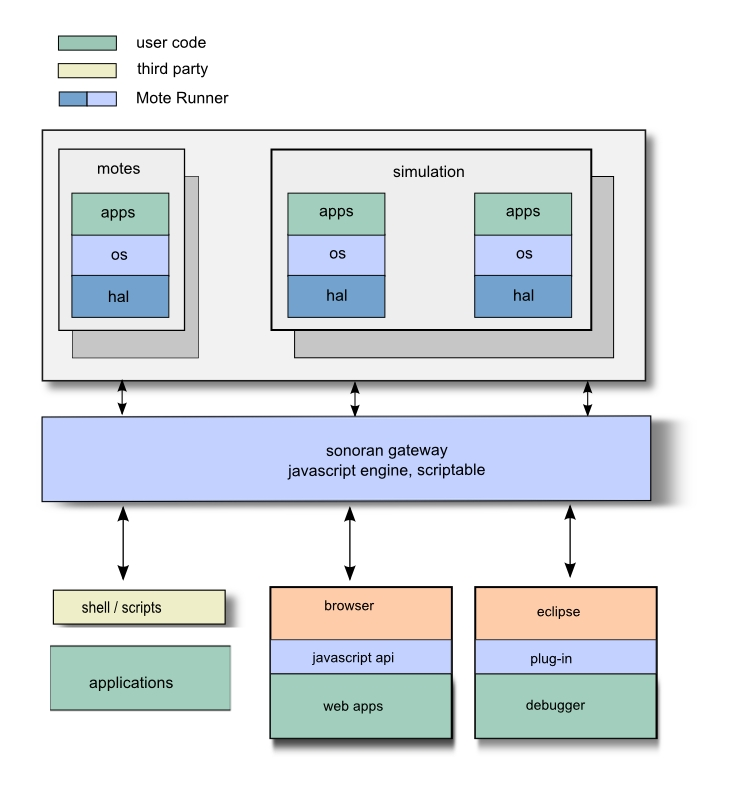
\includegraphics[width=\textwidth]{img/overview.jpg}
    	\end{figure}
    \end{column}
    \hfill
    \begin{column}{.5\linewidth}
    	\begin{figure}
	  \centering
	  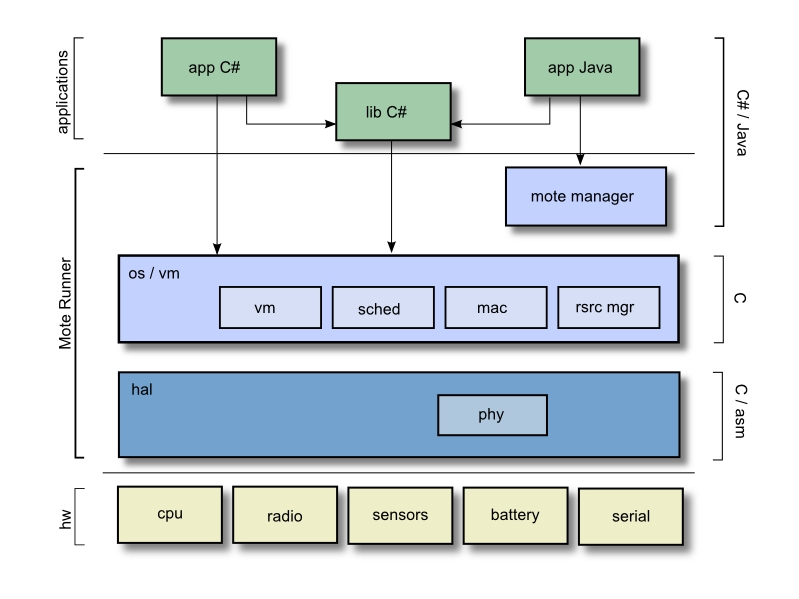
\includegraphics[width=\textwidth]{img/onmote.jpg}
    	\end{figure}
    \end{column}
  \end{columns}
\end{frame}

\begin{frame}[fragile]
  \frametitle{Mote Runner - v.11, v.13 beta}
  \begin{itemize}
    \item They support IEEE 802.15.4
    \begin{itemize}
    	\item exposing a low radio level API that can be used to implement custom MAC layer
    	\item dropping messages with header structure not 802.15.4 compliant in the radio stack 
    \end{itemize}
    \item Offer Hopi
    \begin{itemize}
    	\item A multi-hop data gathering protocol
    	\item Used to collect data from motes setting automatically a tree network
    \end{itemize}
  \end{itemize}
\end{frame}

\begin{frame}[fragile]
  \frametitle{Mote Runner - v.17.1.8c (latest)}
  \begin{itemize}
    \item Supports only two platforms: IMST \& Blipper
    \item It’s based on a different radio layer: LoRa\texttrademark
    \item It offers a build-in MAC layer: LRSC - Low Range Signaling \& Control
    \begin{itemize}
    	\item It supports only a network topology: the LRSC one
    	\item The offered API is poor since the radio is hidden in the firmware (not compatible with previous versions)
    \end{itemize}

  \end{itemize}
\end{frame}

\begin{frame}[fragile]
  \frametitle{LRSC - Architecture}
  \begin{columns}
    \begin{column}{.48\linewidth}
    	\begin{itemize}
	  \item Gateways (GW) are connected to server on IP
	  \item Motes comunicate with server in tunneling TCP/UDP over IP
	  \item Motes comunicate with GW with LoRa single-hop
    	\end{itemize}
    \end{column}
    \hfill
    \begin{column}{.48\linewidth}
    	\begin{figure}
	  \centering
	  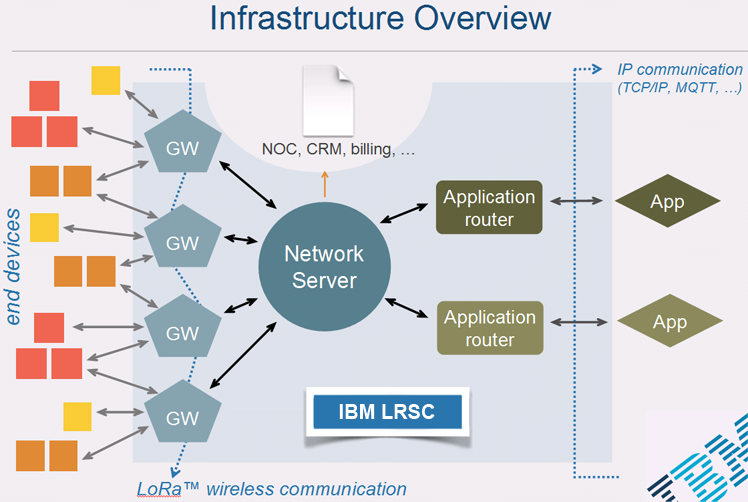
\includegraphics[width=\linewidth]{img/LRSC_infrastructure.png}
    	\end{figure}

    \end{column}
  \end{columns}
\end{frame}

\begin{frame}[fragile]
  \frametitle{LoRa\texttrademark}
  \begin{columns}
    \begin{column}{.48\linewidth}
      \begin{itemize}
	\item LoRa\texttrademark Alliance
	\begin{itemize}
	  \item Target: IoT,  machine-to-machine (M2M), smart city, and industrial applications
	  \item Intiated to standardize Low Power Wide Area Networks (LPWAN)
	\end{itemize}
      \end{itemize}
    \end{column}
    \hfill
    \begin{column}{.48\linewidth}
    	\begin{figure}
	  \centering
	  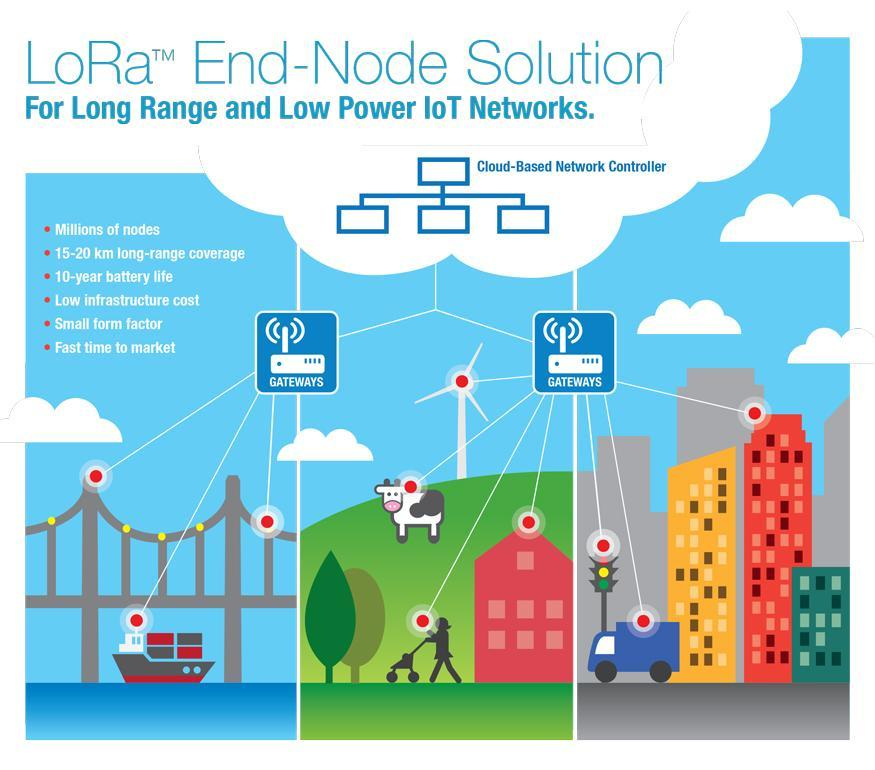
\includegraphics[width=\linewidth]{img/lora.jpg}
    	\end{figure}

    \end{column}
  \end{columns}
\end{frame}

\begin{frame}[fragile]
  \frametitle{LoRa\texttrademark}
  \begin{itemize}
    \item LoRa\texttrademark Technology
    \begin{itemize}
      \item LoRaWAN pledeges to extend the radio range by 10x while using only one third of the power used by competing solutions 
      \item Star (of stars?) topology
      \item Gateways relay messages between end-devices and a central network server
      \item Communication between end-devices and gateways is spread out on different frequency channels and data rates.
      \item Data rates: 0.3 - 50 kbps
    \end{itemize}
  \end{itemize}
\end{frame}

\begin{frame}[fragile]
  \frametitle{LoRa\texttrademark}
  \begin{itemize}
    \item ...and more
    \begin{itemize}
      \item adaptive data rate (ADR)
      \item secure communication (on network and application layers and end-point device key)
      \item three classes of end-point devices.
      \item More info on http://lora-alliance.org/
    \end{itemize}
  \end{itemize}
\end{frame}

\begin{frame}[fragile]
  \frametitle{Mote Runner - Conclusion}
  \vspace{-1em}
  \begin{itemize}
    \item For the purpose of this work (TAKS \& WIDS):
    \begin{itemize}
    	\item MR allows dynamic reprogramming of motes with a control server using WLIP
    	\item v.17.1.8c is not suitable
    	\begin{itemize}
	  \item LoRa is available only for a limited number of platforms (until now!)
	  \item LRSC doesn’t permit to customize the MAC behaviour
	  \item The radio is not exposed
    	\end{itemize}
    	\item v.11, v.13 are better choices:
    	\begin{itemize}
	  \item radio interface could be used to implement an 802.15.4 MAC with TAKS support
	  \item this MAC could be used to build upper layer with WIDS
    	\end{itemize}
    \end{itemize}
    \item This does not exclude a future integration with LoRa-LRSC
  \end{itemize}
\end{frame}

\begin{frame}[fragile]
  \frametitle{Mote Runner}
  \begin{itemize}
  	\item 
  \end{itemize}
\end{frame}
\section{LoRaWAN}
  
\begin{frame}[fragile]
  \frametitle{A deeper look at LoRa}
  \begin{itemize}
      \item LoRaWAN is a Low Power Wide Area Network (LPWAN) specification intended for wireless battery operated Things in regional, national or global network. 
      \item LoRaWAN target key requirements of internet of things:
      \begin{itemize}
      	\item secure bi-directional communication
      	\item mobility - Non molto materiale se non quello su ADR
      	\item localization services - INDAGARE(Beaconing)
      \end{itemize}
  \end{itemize}
\end{frame}

\begin{frame}[fragile]
  \frametitle{LoRa devices sync}
  For time synchronization gateways periodically broadcast so-called beacons. Each beacon
  minimally contains:
  \begin{itemize}
      \item available channels (ChMask)
      \item current GPS time (Time)
      \end{itemize}
      The broadcasting of beacons (in implicit mode) is done time-synchronously (BEACON\_INTERVAL) by all gateways of a network with no interference.
      \begin{figure}
  \centering
  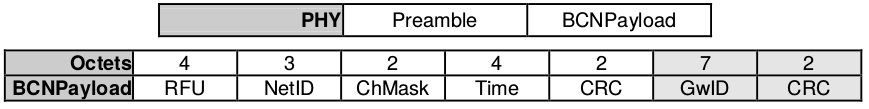
\includegraphics[width=\textwidth]{img/lora_beaconing.png}
  \end{figure}
\end{frame}

\begin{frame}[fragile]
  \frametitle{LoRa MAC Payload Frame}
  \begin{columns}
    \begin{column}{.48\linewidth}
    LoRa MAC message types:
       \begin{itemize}
        \item join request
        \item join accept 
        \item unconfirmed data messages
        \item confirmed data messages
       \end{itemize}
  \end{column}
   \begin{column}{.48\linewidth}
 \begin{figure}
  \centering
  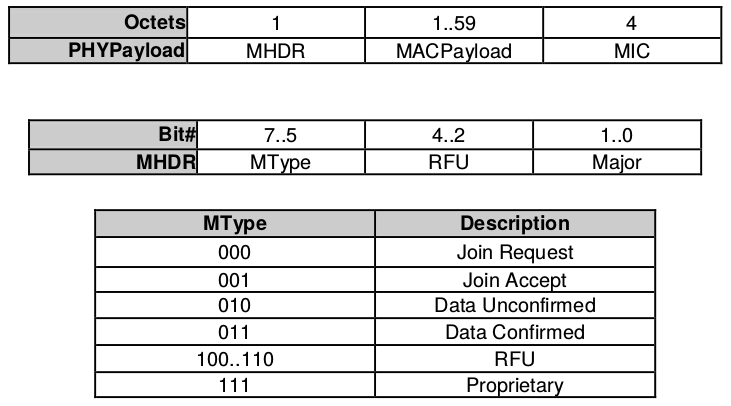
\includegraphics[width=\textwidth]{img/mac_frame.png}
  \end{figure}
  \end{column}
  \end{columns}
\end{frame}

\begin{frame}[fragile]
  \frametitle{LoRa end-devices}
  \begin{itemize}
   \item  Release v1.0 allows at MAC and Application layers, Bi-directional communications:
     \begin{itemize}
       \item Class A: after send operation two tiny time windows are opened in order to allow reception
       \item Class B: send and receive operations may be scheduled based on the time information contained in the beacons
     \end{itemize}
    \item  Last Release = Release v1.0 plus:
     \begin{itemize}
       \item Class C: nearly continuously open receive windows, only closed when transmitting.
     \end{itemize}
  \end{itemize}
  \begin{figure}
  \centering
  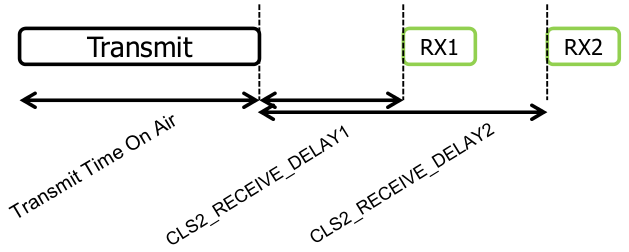
\includegraphics[width=0.4\textwidth]{img/lora_rx_windows.png}
  \end{figure}

\end{frame}


\begin{frame}[fragile]
  \frametitle{LoRa secure communications - 1}
  In order to partecipate in a LoRa network an end device first has to be personalized and the activated.
  Activation of an end device can be achieved in two ways:
  \begin{itemize}
    \item OTAA (over-the-air activation) when an end device is deployed or reset;
    \item APB (activation by personalization) one-step personalization and activation.
  \end{itemize}
\end{frame}

\begin{frame}[fragile]
  \frametitle{LoRa secure communications - 2}
  During activation the end device holds the following informations:
  \begin{itemize}
      \item \textbf{DevAddr:} device ID of 32 bits that uniquely identifies the end device.
      \item \textbf{AppEUI:} globally unique application ID that uniquely identifies the application provider of the end device.
      \item \textbf{NwkSKey:} device-specific network session key, ensures data integrity and os used to encrypt/decrypt MAC data messages payload
      \item \textbf{AppSKey:} device-specific application session key, used to encrypt and decrypt the payload field of application-specific data messages.
  \end{itemize}
\end{frame}


\begin{frame}[fragile]
  \frametitle{LoRa secure communications - OTAA}
 \begin{figure}
  \centering
  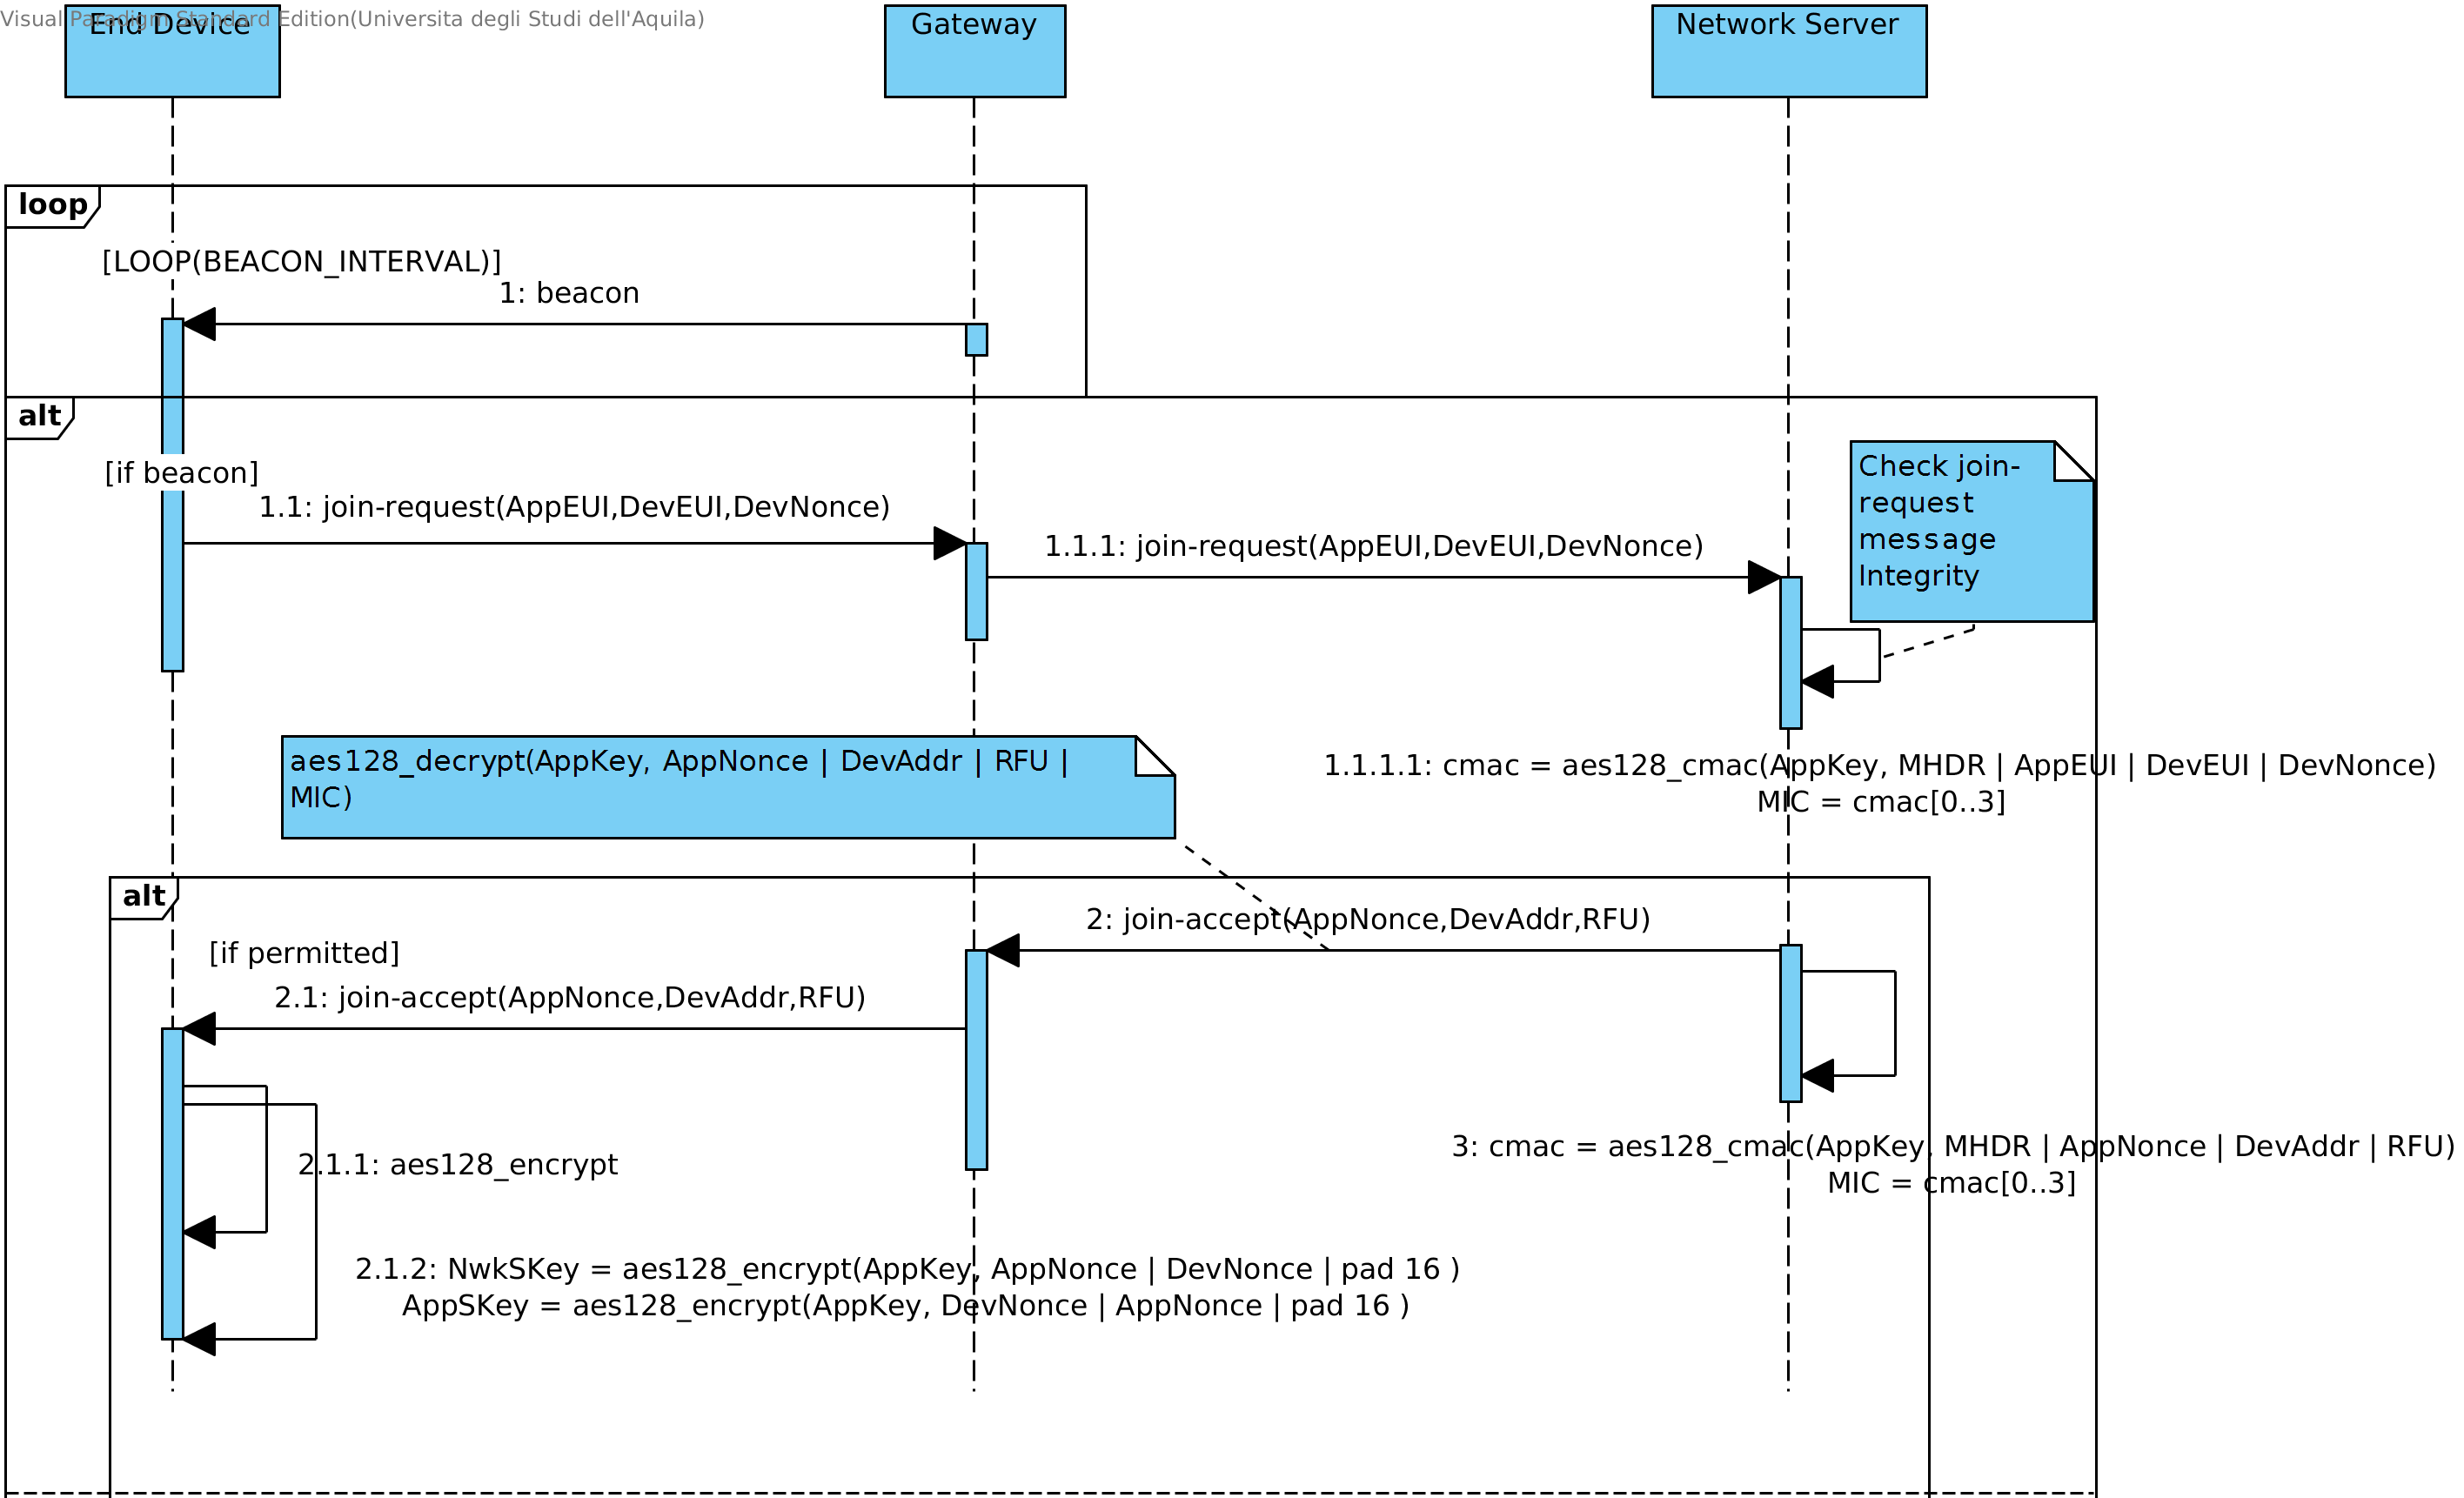
\includegraphics[width=0.9\textwidth]{img/lora_secure.png}
  \end{figure}
\end{frame}

\begin{frame}[fragile]
  \frametitle{LoRa mobility}
  LoRa network data rates are:
 \begin{itemize}
  \item Network controlled for fixed devices by means of using ADR bit in the PHY payload of data messages:
  \begin{itemize}
    \item If is set, the network will control the data rate of the end device through the appropriate MAC commands
    \item If is cleared, the network will not attempt to control the data rate of the end device independently of the received signal quality
  \end{itemize}
  \item default for mobile end-devices.
\begin{figure}
  \centering
  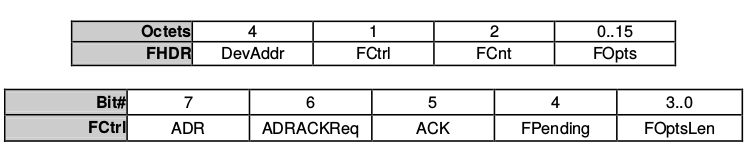
\includegraphics[width=0.9\textwidth]{img/PHYpayload.png}
  \end{figure}
 \end{itemize}

\end{frame}

\begin{frame}[fragile]
  \frametitle{LoRa mobility 2}
 \begin{itemize}
  \item \hypertarget{refthis}{}
  \item However, whenever possible, the ADR scheme should
be enabled to increase the battery life of the end device and maximize the network capacity
 \end{itemize}

\end{frame}
\section{Physical layer in \mbox{Mote Runner}}
\begin{frame}[fragile]
  \frametitle{Radio interface - 1}
  \begin{itemize}
    \item MR v.13 offers a Radio interface IEEE 802.15.4 compliant
    \begin{itemize}
    	\item It is a generic class in the IBM saguaro system that permits to use the radio device
    	\item It offers an API with the following functionality:
    	\begin{itemize}
			\item open: opens the radio, once opened no other assembly can use it
			\item close: releases the radio so that others can use it
			\item setter and getters for channel and network parameters (addresses, panid...)
			\item startReceive: listens the channel (in one of the many receiption mode)
			\item transmit: begin to transmit a pdu
    	\end{itemize}
    \end{itemize}
  \end{itemize}
\end{frame}

\begin{frame}[fragile]
	\frametitle{Radio interface - 2}
	\begin{itemize}
		\item In addition Radio:
		\begin{itemize}
			\item Handles transmission and reception notifying to higher level by delegation, registering functions that will handle the events (tx and rx)
			\item Manages acks notifying states of failure or success to callbacks
			\item Permits to set parameters as PAN identifier, short address, radio channel
		\end{itemize}
	\end{itemize}
\end{frame}


\begin{frame}[fragile]
  \frametitle{Transmission \& Reception - 1}
  \begin{itemize}
    \item These operations require much attention:
    \begin{itemize}
    	\item Radio permits to transmit every type of pdu, but it's possible to receive only packets with 802.15.4 well formed headers
    	\item Receiving in promiscuous mode allows to receive every kind of packet, but this exposes to interferences
    \end{itemize}
    \item Each mote holds 3 addresses:
    \begin{itemize}
    	\item a 16-bit PAN identifier
    	\item a 64-bit extended address that uniquely identifies a mote (EUI-64)
    	\item a 16-bit short address that's application and protocol specific
    \end{itemize}
  \end{itemize}
\end{frame}

\begin{frame}[fragile]
  \frametitle{Transmission \& Reception - 2}
  \begin{figure}
  	\centering
  	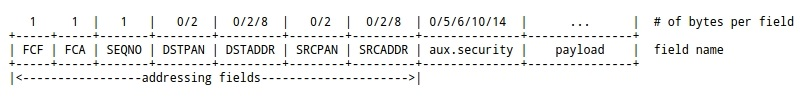
\includegraphics[width=\textwidth]{img/header.jpg}
  	\caption{PDU header format}
  \end{figure}
  \begin{columns}
  	\begin{column}{.52\textwidth}
	    \begin{figure}
	    	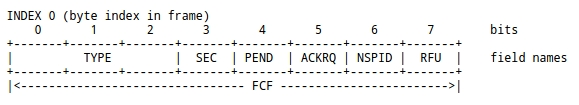
\includegraphics[width=\textwidth]{img/fcf.jpg}
  		\caption{Frame Control Flags}
	    \end{figure}
  	\end{column}
  	\hfill
	\begin{column}{.45\textwidth}
	    \begin{figure}
	    	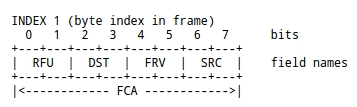
\includegraphics[width=\textwidth]{img/fca.jpg}
  		\caption{Frame Control Address Flags}
	    \end{figure}
  	\end{column}
  \end{columns}
\end{frame}
% 
% \begin{frame}[fragile]
%   \frametitle{Tx/Rx - Filtering}
%   \begin{itemize}
%     \item Possible packets are specified in FCF-Type field and are: BEACON, DATA, ACK and CMD.
%     \item BEACONs are accepted only if the header field SRCPAN matches the mote's PANID or it's BROADCAST
%     \item If FCA Flags specify an address then 
%   \end{itemize}
% \end{frame}

\begin{frame}[fragile]
  \frametitle{Tx/Rx and Real Time Constraints}
  \begin{itemize}
    \item It's possible to operate in many different ways with regards to real time constraints:
    \begin{itemize}
    	\item ASAP, EXACT, TIMED, RX4EVER indicate when the operation should begin and/or end given two time instant
    	\item MR manages autonomously all warm up and ramp up to make the device ready given one of these modes
    	\item At the end the device turns off and an event is raised to be managed with delegation
    	\item If the device cannot be ready or cannot complete a task within the specified time an error occurs
    \end{itemize}
  \end{itemize}
\end{frame}
\section{A MAC Layer in Mote Runner}
\begin{frame}[fragile]
  \frametitle{Coming soon}
  
\end{frame}
\section{6LoWPAN implementation in \mbox{Mote Runner}}
\begin{frame}[fragile]
  \frametitle{Introduction to 6LoWPAN}
  \begin{figure}
    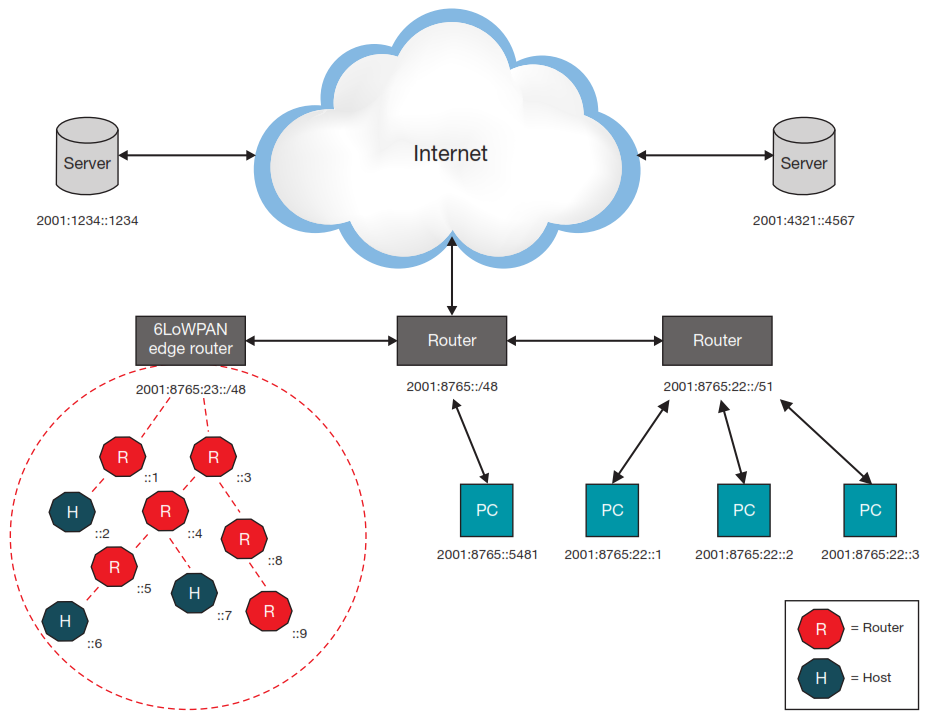
\includegraphics[width=.7\textwidth]{img/6low_network.png}
    \caption{IPv6 network with a 6LoWPAN mesh network}
  \end{figure}
\end{frame}

\begin{frame}[fragile]
  \frametitle{6LoWPAN stack}
  \begin{figure}
    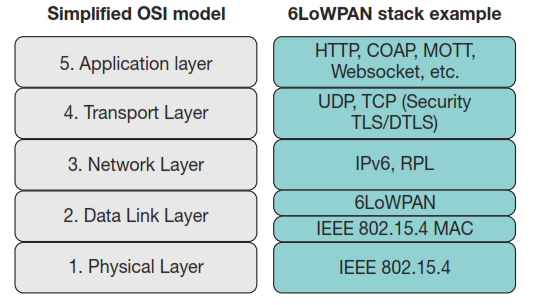
\includegraphics[width=.6\textwidth]{img/6low_stack.png}
  \end{figure}
\end{frame}

\begin{frame}[fragile]
  \frametitle{MRv6: an implementation of 6LoWPAN in MR}
  \begin{itemize}
    \item TDMA and beacon based multi-hop network which allows for an IPv6 based communication between motes
    \item It is not a built-in MR component, but it is fully implemented in C\#
    \item Datagram packets exchanged adheres to a subset of the 6LoWPAN specifications
    \item The edge mote decides upon:
    \begin{itemize}
      \item Association requests
      \item Assigns communication schedules between wireless nodes
      \item Determines the routes in the network
    \end{itemize}
  \end{itemize}
\end{frame}

\begin{frame}[fragile]
  \frametitle{MRv6: Limitations}
  \begin{itemize}
    \item Only the transmission of UDP packets within the 6LoWPAN network is supported
    \item Exists only a proprietary broadcast operation to reach all motes in the network
    \item Is not suited for low latency application
    \item Does not support packet segmentation, reassembly and flow control
    \item Has been deployed in 900MHz or 2.4GHz frequency ranges and uses a single channel in the 2.4GHz band yet
  \end{itemize}
\end{frame}

\begin{frame}[fragile]
  \frametitle{Scheduling}
  \begin{itemize}
    \item The network tree is only know to the edge
    \item The communication slots between parent and children are globally assigned by the edge and do never overlap
    \end{itemize}
    \begin{table}[h]
      \begin{tabular}{@{}|c|c|l|l|l|l|@{}}
	\toprule
	 SF edge & SF mote 1 & SF mote 2 & ... & SF max mote \\ \bottomrule
      \end{tabular}
    \end{table}
\end{frame}

\begin{frame}[fragile]
  \frametitle{Superframe}
  \begin{itemize}
   \item At the beginning of their communication period parent motes send out beacon messages
    \item Other then a fixed exclusive slot, parent offers a shared slot (e.g. association requests and responses, broadcast messages)
    \item Beacon, shared and fixed slots form the superframe whose timings are assigned by the edge
  \end{itemize}
  \begin{table}[h]
    \begin{tabular}{@{}|p{1.5cm}|p{1.5cm}|p{1.5cm}|p{1cm}|p{1.5cm}|p{1cm}|@{}}
      \toprule
      Beacon slot & Shared slot & Child slot 0 & ... & Child slot n & Gap \\ \bottomrule
    \end{tabular}
  \end{table}
\end{frame}

\begin{frame}[fragile]
  \frametitle{Association}
  \begin{itemize}
    \item The joining mote evaluates information in the beacons (e.g. number of children or hops to the edge)
    \item Mote sends and association request in the shared slot of the potential parent
    \item Parent forward the request to the edge with the EUI-64 of the joining mote
    \item When the edge accepts the mote:
    \begin{itemize}
      \item It allocates short address and superframe timings for the mote
      \item The parent forwards the response to the new child in its shared slot and adds it to its list
    \end{itemize}
  \end{itemize}
\end{frame}

\begin{frame}[fragile]
 \frametitle{Short comparison}
 \begin{table}[h]
    \begin{tabular}{@{}p{5cm}|p{5cm}@{}}
      \toprule
      Our Mac-Like &  MRv6 \\ \midrule
      Contention based &  Scheduled\\
      \hline
      Transmit only when  \mbox{requested} &  S-TDM\\
      \hline
      Association managed by pan-coordinator & Association managed by the edge  \\ 
      ... & ... \\ \bottomrule
    \end{tabular}
  \end{table}
\end{frame}

\section{Conclusions} 
\begin{frame}[fragile]
  \frametitle{TODO}
\end{frame}

\section{Integrazione LoRa}

\begin{frame}[fragile]
  \frametitle{LoRaWAN Classes}
  \begin{figure}
    \centering
    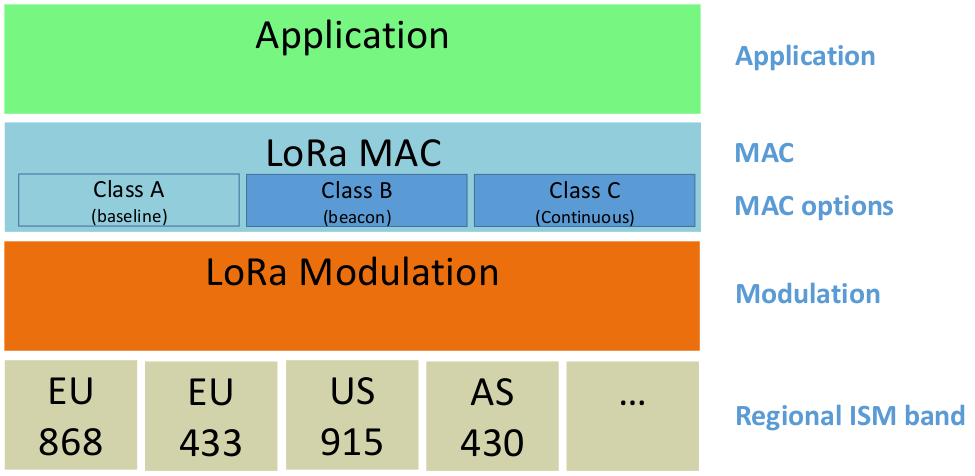
\includegraphics[width=0.9\textwidth]{img/loraClasses.png}
  \end{figure}
\end{frame}


\begin{frame}[fragile]
  \frametitle{Class A end-devices}
  \begin{itemize}
    \item Its funtionalities are implemented by every end-device.
    \item Uplink: devices transmit following Aloha method.
    \item Downlink: after a transmission two tiny time windows are opened to allow reception
    \begin{itemize}
      \item RX1 uses the same frequency channel as the uplink and a data rate depending on the one in the uplink;
      \item RX2 uses a fixed configurable frequency and data rate;
      \item Devices is active in rx only if a preamble is detected.
    \end{itemize}
  \end{itemize}
  \begin{figure}
		\centering
		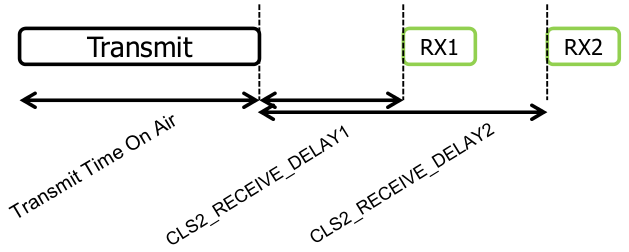
\includegraphics[width=0.4\textwidth]{img/lora_rx_windows.png}
  \end{figure}
\end{frame}

\begin{frame}[fragile]
  \frametitle{Class B end-devices}
  \begin{itemize}
		\item Class B end-devices are optimized for mobile and fixed battery-powered end-devices.
		\item They add a synchronized reception window called ``ping slot''
		\begin{itemize}
			\item Synchronization requires beacons;
			\item Devices selects randomly a ping slot at each beacon to avoid collisions.
		\end{itemize}
	\end{itemize}
	\begin{figure}
		\centering
		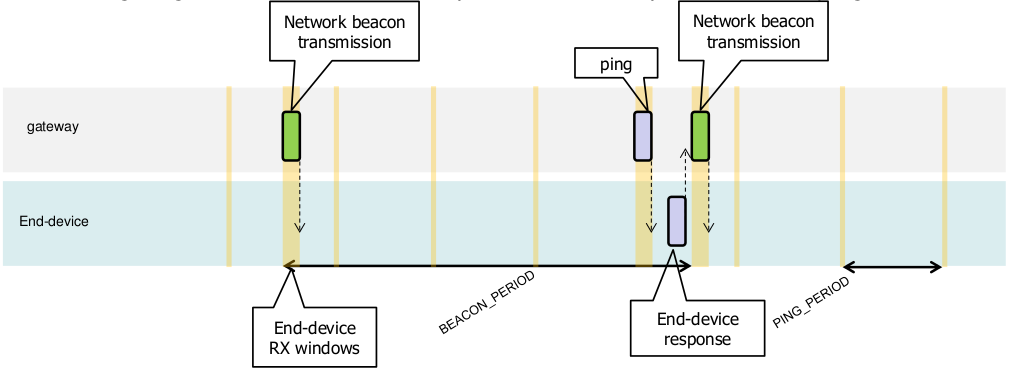
\includegraphics[width=0.8\textwidth]{img/loraBeacon.png}
	\end{figure}
\end{frame}

\begin{frame}[fragile]
  \frametitle{Class B end-devices}
  \begin{itemize}
		\item All end-devices start and join the network as end-devices of Class A.
		\item The end-device application can then decide to switch to Class B.
		\item The end-device waits a beacon and selects a ping slot of 30 ms from the 4096 available in a beacon interval.
		\item When the mote is far from BS the duration is extended, if beacon is not received the device tries to mantain the synchronization for 2 hours after that it returns to class A
  \end{itemize}
\end{frame}

\begin{frame}[fragile]
	\frametitle{Class C end-devices}
	\begin{itemize}
		\item This mode is used when there are no need for energy awareness and there's no need to minimize reception time.
		\item Class C end-devices cannot implement Class B option.
		\item These devices will listen with RX2 windows parameters as often as possible.
	\end{itemize}
	\begin{figure}
		\centering
		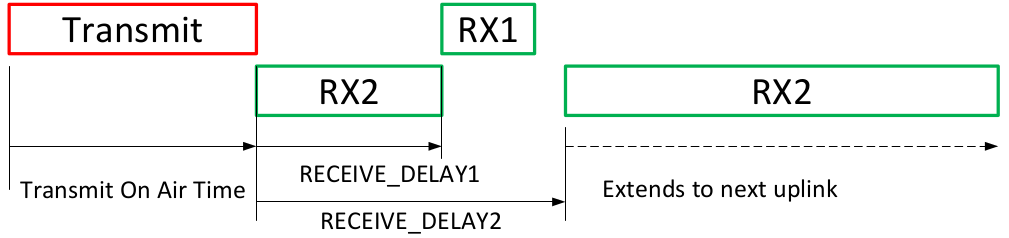
\includegraphics[width=0.8\textwidth]{img/loraClassC.png}
	\end{figure}
\end{frame}


\end{document}
